\documentclass{article}
\usepackage{graphicx} % Required for inserting images
\usepackage{authblk} % Required for author affiliations
\usepackage{indentfirst} % Indent first paragraph of sections
\usepackage{amssymb} % For mathematical symbols
\usepackage{amsthm} % For theorem environments
\usepackage{amsmath} % For advanced math typesetting
\usepackage[hidelinks]{hyperref}
\usepackage{enumitem}
\usepackage{pgfplots} % For plots
\usetikzlibrary{arrows.meta,calc}
\pgfplotsset{compat=1.18} % Set compatibility level
\usepackage{tikz} % For drawing shapes
\newtheorem{theorem}{Theorem}
\newtheorem{corollary}{Corollary}[theorem]
\newtheorem{lemma}[theorem]{Lemma}
\newtheorem{definition}{Definition}
\newtheorem{problem}{Problem}
\newtheorem{solution}{Solution}
\newtheorem*{example}{Example}
\newtheorem{remark}{Remark}
\reversemarginpar
\begin{document}
%------- Title page   -----------
\title{MATH 223: Linear Algebra}
\author{William Homier}
\affil[1]{McGill University Physics, 3600 Rue University, Montréal, QC H3A 2T8, Canada}
\date{January \(5^{th}\), 2026}
\setcounter{Maxaffil}{0}
\renewcommand\Affilfont{\itshape\small}
\maketitle

%------- Abstract -----------
\noindent\rule{\textwidth}{0.4pt}
\thispagestyle{empty}
\begin{abstract}

\end{abstract}
\noindent\rule{\textwidth}{0.4pt}
\clearpage

%------- Table of Contents -----------
\thispagestyle{empty}
\hypersetup{
    citecolor=black,
    filecolor=black,
    linkcolor=black,
    urlcolor=black
}
\tableofcontents
\clearpage

%------- introduction -----------
\setcounter{page}{1}
\section{Introduction}

\section{Prerequisite knowledge}
\subsection{Notation}
\subsubsection{Sets}
Sets are a grouping of objects.
\begin{center}
\begin{tabular}{c|p{6cm}|p{5cm}}
Set & Meaning & Examples \\
\hline
$\mathbb{N}$ & The set of natural numbers & (0, 1, 2, 3, ...)\\
$\mathbb{Z}$ & The set of integers & (..., -3, -2, -1, 0, 1, 2, 3, ...)\\
$\mathbb{Q}$ & The set of rational numbers & \(\mathbb{Q} = {\frac{a}{b}\:|\:\forall a,b \in \mathbb{Z}\:and\:b \neq 0}\)\\
$\mathbb{R}$ & The set of all rational and all irrational numbers & \((...,-1,0,\frac{1}{4},1,1000,...)\)\\
$\mathbb{C}$ & The set of all complex numbers & \(\mathbb{C} = \{x + iy\:|\:x,y \in \mathbb{R}\:and\:i \subseteq \sqrt{-1}\}\).\\
\end{tabular}
\end{center}

We have the following relationships between sets:
\[\mathbb{N} \subseteq \mathbb{Z} \subseteq \mathbb{Q} \subseteq \mathbb{R} \subseteq \mathbb{C}\]
\subsubsection{Symbols}
\begin{center}
\begin{tabular}{c|l}
Symbol & Meaning \\
\hline
$\subseteq$ & is a subset of or equal to \\
$\subset$ & is a strict subset of \\
$\in$ & is an element of \\
$\forall$ & for all \\
$\exists$ & there exists \\
$\emptyset$ & empty set \\
$\Rightarrow$ & implies \\
$\Leftrightarrow$ & if and only if
\end{tabular}
\end{center}

\subsection{Complex Algebra}
\subsubsection{Complex Numbers}
A complex number is of the form: \(z = x + iy\) where \(x,y \in \mathbb{R}\) and \(i\) is the imaginary unit such that \(i^2 + 1 = 0\).
\begin{definition}[Powers of \(i\)]
\begin{tabular}{c|cccccc}
k & 0 & 1 & 2 & 3 & 4 & 5 \\
\hline
$i^k$ & 1 & i & -1 & -i & 1 & i
\end{tabular}
\end{definition}
\begin{theorem}[Fundamental Theorem of Algebra]
    Any complex polynomial\footnote{Polynomial is a function such as: \(f = a_n x^n + a_{n-1}x^{n-1} + ... + a_1 x + a_0\) where \(a_i \in \mathbb{R}\) or \(\mathbb{C}\) and \(n \in \mathbb{N}\).} \(f\) (except constant functions) has a root in \(\mathbb{C}\).
\end{theorem}
\begin{remark}
    If we have a polynomial \(f\) of degree \(n\), then it has \(n\) roots, where each root can have a multiplicity\footnote{The multiplicity of a root represents how many times the root occurs in the polynomial.}.
\end{remark}
\begin{example}
    If we have a polynomial \((x-1)^2\), it has a degree of 2 but only one root, which is 1, with a multiplicity of 2. This means that the root 1 appears twice in the polynomial.
\end{example}
We can factorize a polynomial in the form of \(f = a_n x^n + ... + a_1 x + a_0\) into a linear factor: \(f = a(x - z_1)(x - z_2)...(x - z_n)\) where \(z_i\) are the roots of \(f\) in \(\mathbb{C}\).\\\\
Using the FTA for a function such as \(f = a_nx^n + ... + a_1 x + a_0\), we can say that the FTA implies that \(f\) has a root \(f(z) = 0\), because $f(z) = a(z-z) = 0$.
\subsubsection{Complex Operations}
\label{subsec:CO}
We can define operations on complex numbers as follows:
\begin{itemize}
    \item Addition: \(z + z' = (x + x') + i(y + y')\), where \(x,x',y,y' \in \mathbb{R}\).
    \item Multiplication: \(zz' = (x + iy)(x' + iy') = (xx' - yy') + i(xy' + yx')\).
    \item Inverse: \(\frac{1}{z} = \frac{\overline{z}}{z\overline{z}} = \frac{x - iy}{x^2 + y^2} = \frac{x}{x^2 + y^2} + i\frac{-y}{x^2 + y^2}\)
\end{itemize}
From the definition of inverse, we can see that for any complex number \(z\), its inverse \(\frac{1}{z}\) is also a complex number. For example, take \(z = 1 + i\), where \(x = y = 1\), from the definition of inverse, we can conclude that:
\[\frac{1}{1 + i} \in \mathbb{C}\]
Multiplying by a complex number \(z\) corresponds geometrically to
\[\begin{cases}\text{a rotation by some angle } \theta,\\\text{a rescaling by the factor } |z|.\end{cases}\]
\subsubsection{Complex Conjugate}
A complex conjugate is a way to "flip" the imaginary part of a complex number. For example, if we have a complex number \(z = x + iy\), then the complex conjugate of \(z\) is \(\overline{z} = x - iy\). Some basic properties of complex conjugates are:
\begin{itemize}
    \item \(\overline{z} = z\)
    \item \(\overline{z + z'} = \overline{z} + \overline{z'}\)
    \item \(\overline{z \cdot z'} = \overline{z} \cdot \overline{z'}\)
\end{itemize}

\subsubsection{Geometric and Polar Form of Complex Numbers}
\marginpar{January 09, 2026.}

\paragraph{1. Geometric Interpretation}
\begin{definition}[Geometric interpretation]
    Every complex number \(z = x + iy\) can be identified with a point \((x,y)\) in the plane, called the complex plane.
\end{definition}
We define the complex plane as:
\[\mathbb{C} = \{x + iy \mid x,y \in \mathbb{R}\}.\]

\begin{center}
\begin{tikzpicture}[scale=2]
% Axes
\draw[->] (-1.4,0)--(1.4,0) node[right]{$x$};
\draw[->] (0,-1.4)--(0,1.4) node[above]{$y$};

% Unit circle
\draw (0,0) circle(1);

% Point z = x+iy
\coordinate (Z) at (0.8,0.6);
\draw[fill] (Z) circle(0.02) node[above right] {$z=x+iy$};

% Projections
\draw[dashed] (Z) -- (0.8,0) node[below] {$x$};
\draw[dashed] (Z) -- (0,0.6) node[left] {$y$};

% Horizontal from y-axis and vertical from x-axis
\draw (0,0.6) -- (Z);
\draw (0.8,0) -- (Z);

% Radius
\draw (0,0) -- (Z);

\end{tikzpicture}
\end{center}

\paragraph{2. Modulus and Unit Circle}
\begin{definition}[Modulus]
    The modulus of a complex number \(z\) is defined by
    \[|z| = \sqrt{z\overline{z}} = \sqrt{x^2 + y^2}.\]
    Geometrically, \(|z|\) is the distance from the origin to the point \((x,y)\).
\end{definition}
We can rewrite the definition of the unit circle as follows:
\[S' = \{(x,y) \in \mathbb{R}^2 : x^2 + y^2 = 1\} = \{ z \in \mathbb{C} : |z| = 1\},\]
where \(S'\) is the unit circle in the complex plane.

\paragraph{3. Polar Coordinates}

\begin{definition}[Polar coordinates]
    Instead of describing a point by \((x,y)\), we may describe it using polar coordinates \((r,\theta)\), where \(r = |z|\) is the distance to the origin and \(\theta\) is the angle with the positive \(x\)-axis.
\end{definition}
\begin{example}
    Consider the point \((x,y)\), where \(x = r \cos(\theta)\:and\:y = r \sin(\theta)\). We can define \((r,\theta)\) as follows:
    \begin{center}
    \begin{tikzpicture}[scale=2]
    % Axes
    \draw[->] (-1.4,0)--(1.4,0) node[right]{$x$};
    \draw[->] (0,-1.4)--(0,1.4) node[above]{$y$};

    % Point
    \coordinate (Z) at (0.9,0.5);
    \draw[fill] (Z) circle(0.02) node[above right] {$(x,y)$};

    % Lines
    \draw (0,0) -- (Z) node[midway, above] {$r$};
    \draw[dashed] (Z) -- (0.9,0);
    \draw[dashed] (Z) -- (0,0.5);

    % Angle theta
    \draw (0.4,0) arc (0:29:0.4);
    \node at (0.45,0.12) {$\theta$};

    \end{tikzpicture}
    \end{center}
\end{example}
Complex numbers can also be described using polar coordinates.
\begin{definition}[Polar and exponential form]
    \[z = x + iy = r \cos(\theta) + ir \sin(\theta) = r(\cos(\theta) + i \sin(\theta)) = re^{i\theta}.\]
\end{definition}
We can also define multiplication in polar form:
\begin{definition}[Multiplication in polar form]
    \[z = re^{i\theta}, \quad z' = r'e^{i\theta'}, \quad zz' = rr'e^{i(\theta + \theta')}.\]
\end{definition}
\begin{example}
    \[(1 + i)^{32} = (\sqrt{2}e^{i\pi/4})^{32} = (\sqrt{2})^{32} e^{i8\pi} = 2^{16}(\cos 8\pi + i \sin 8\pi) = 2^{16}.\]
\end{example}

Around the 1740, the mathematician Euler discovered a formula for complex numbers. The formula is known as Euler's formula.
\begin{definition}[Euler's formula]
    \[e^{i\theta} = \cos(\theta) + i \sin(\theta).\]
\end{definition}
This formula is quite useful when dealing with complex numbers, as it allows us to write complex numbers in a more compact form.

\paragraph{4. Roots in $\mathbb{C}$}
\begin{definition}[\(n^{\text{th}}\) roots in $\mathbb{C}$]
    For any complex number $z$, an $n^{\text{th}}$ root of $z$ is a complex number $w$ such that
    \[w^n = z.\]
\end{definition}
\begin{example}
    If \(z = re^{i\theta}\), then any solution of \(w^n = z\) must satisfy
    \[w_k = r^{1/n} e^{i(\theta + 2\pi k)/n}, \quad k = 0,1,2,\dots,n-1,\]
    where the $n^{\text{th}}$ roots of $z$ are equally spaced on a circle of radius $r^{1/n}$ centered at the origin.
\end{example}
\begin{definition}[Roots of unity]
The \(n^{\text{th}}\) roots of unity are the solutions of a special case where $z = 1$.
\end{definition}
\begin{example}
    If $z = 1$, then any solution of $w^n = z$ must satisfy
    \[w_k = e^{i2\pi k/n}, \quad k = 0,1,2,\dots,n-1.\]
    Geometrically, they lie on the unit circle and are equally spaced.
\end{example}

\section{Basic Algebraic structures}
\subsection{Sets with Multiplication}
\begin{definition}[Set with multiplication]
A set $M$ is called a set with multiplication if you can multiply any two elements of $M$, and the result is still in $M$.
In other words, for any $a,b \in M$, the product $ab$ is also in $M$.
\end{definition}
\begin{example}
Let $M = \mathbb{R}$.  
If $a,b \in \mathbb{R}$, then $ab \in \mathbb{R}$.  
So the real numbers $\mathbb{R}$ form a set with multiplication.
\end{example}
\begin{example}
    An example of a set with multiplication is the set of all \(2 \times 2\) complex matrices: \(M = M_2(\mathbb{C})\). Another example is the nonzero set of all real numbers \(\mathbb{R}\) with ordinary multiplication: \(\mathbb{R}^* = \mathbb{R} \setminus \{0\}\).
\end{example}

\subsection{Invertibility}
\begin{definition}[Condition for Invertibility]
    Let \(A \in M\) be an \(n \times n\) matrix, and suppose that there exists an \(n \times n\) matrix \(B\) such that \(AB = I_n\) or \(BA = I_n\). Where \(I_n\) is the \(n \times n\) identity matrix\footnote{An identity matrix is a square matrix with 1s on its main diagonal and 0s everywhere else. It represents no change in linear transformations, and it's used in finding matrix inverses.}$\begin{bmatrix}1&0&0\\0&\ldots&0\\0&0&1\end{bmatrix}$. Then A is invertible, and \(B\) is called the inverse of \(A\) and is denoted by \(B = A^{-1}\).
\end{definition}
\begin{remark}
    If \(A\) is invertible, then \(A^{-1}\) exists and is unique\footnote{Unique means there is exactly one such element.}.
\end{remark}

To determine if an element \(A\) in a set with multiplication \(M\) is invertible, we can use the following examples:
\begin{example}
    Let \(M = \mathbb{Z} = \{...-2,-1,0,1,2,...\}\) and \(A = 2\). Is \(A\) invertible in \(M\)?\\
    Solution: No, because \(\frac{1}{2} \notin \mathbb{Z}\).
\end{example}
\begin{example}
    Let \(M = \mathbb{R}\) and \(A = 2\), is \(A\) invertible in \(M\)?\\
    Solution: Yes, because \(\frac{1}{2} \in \mathbb{R}\).
\end{example}
\begin{example}
    Is \(1 + i\) invertible in \(\mathbb{C}\)?\\
    Solution: Yes, using our previous definition of inverse (\ref{subsec:CO}), we get that \[\frac{1}{1 + i} = \frac{1 - i}{2} \in \mathbb{C}.\]
\end{example}

\subsection{Ring}
\begin{definition}
A \textbf{ring} is a set $R$ where you can \textbf{add} and \textbf{multiply} elements, and the following are true:

\begin{enumerate}
    \item You can add any two elements and stay in $R$. There is a zero, every element has a negative, and addition is commutative and associative.
    \item You can multiply any two elements and stay in $R$. Multiplication is associative, and there is a $1$.
    \item Multiplication distributes over addition:
    \[
    a(b+c) = ab + ac \quad \text{and} \quad (a+b)c = ac + bc.
    \]
\end{enumerate}
\end{definition}
The main example of a ring is the set of integers $\mathbb{Z}$.

\subsection{Field} %need to organize
\begin{definition}
    A field is a set of numbers which can be added, subtracted, multiplied, and divided (except for division by zero) in a way that satisfies certain rules. These rules are:
    \begin{enumerate}
        \item You can add any two elements and stay in the field. There is a zero, every element has a negative, and addition is commutative\footnote{} and associative.
        \item You can multiply any two elements and stay in the field. Multiplication is associative, and there is a 1.
        \item Multiplication distributes over addition:
        \[
        a(b+c) = ab + ac \quad \text{and} \quad (a+b)c = ac + bc.
        \]
    \end{enumerate}
    Examples of fields include the real numbers \(\mathbb{R}\) and the complex numbers \(\mathbb{C}\).\\
\end{definition}

\begin{problem}
    Construct a field with 2 elements.
\end{problem}
\begin{problem}
    Show that if an inverse of A in \(\mathbb{M}\) exists, then it is unique.
\end{problem}
\begin{problem}
    Let \(K\) be a field. Prove that this matrix $\begin{bmatrix}0&1\\0&0\end{bmatrix}$ \(\in M_2(K)\) is not invertible.
\end{problem}

\section{Vector Spaces}
\marginpar{January 09, 2026.}
\subsection{Cartesian vector spaces}
\begin{definition}[$R^n$]
Let \(n \in \mathbb{N}\). The Cartesian product of \(n\) copies of \(\mathbb{R}\) is called \(\mathbb{R}^n\).
\[\mathbb{R}^n = \{\begin{pmatrix}x_1\\\ldots\\x_n\end{pmatrix} : x_1, \ldots, x_n \in \mathbb{R}\}\]
\end{definition}

\subsection{Vectors}
\subsubsection{Vector operations}
Vector operations are defined as follows.\\
Addition: \(\begin{pmatrix} x_1 \\ \vdots \\ x_n \end{pmatrix} + \begin{pmatrix} y_1 \\ \vdots \\ y_n \end{pmatrix} = \begin{pmatrix} x_1 + y_1 \\ \vdots \\ x_n + y_n \end{pmatrix}\),\\
scalar multiplication: \(\lambda \begin{pmatrix} x_1 \\ \vdots \\ x_n \end{pmatrix} = \begin{pmatrix} \lambda x_1 \\ \vdots \\ \lambda x_n \end{pmatrix}\), where \(\lambda \in \mathbb{R}\).

\begin{definition}[Linear combination]
    A linear combination of vectors \(v_1, \ldots, v_n\) is a vector \(v\) of the form \(v = \lambda_1v_1 + \ldots + \lambda_nv_n\), where \(\lambda_1, \ldots, \lambda_n \in \mathbb{R}\).
\end{definition}
\begin{example}
    A linear combination could look like this:
    \[\xi((v_1 + 2v_2) + v_3) + v_4,\]
    where $\xi \in \mathbb{R}$.
\end{example}

\subsubsection{Span}
\marginpar{January 12, 2026.}
\begin{definition}[Span]
Let \(A \subset \mathbb{R}^2\). The span of \(A\), denoted \(Span(A)\), is the set of all linear combinations of elements of \(A\).
\end{definition}
\begin{remark}
If \(A = \{v\}\) contains one nonzero vector, then \(\operatorname{Span}(v)\) is a line through the origin.
\end{remark}
\begin{example}
Let \(A = \begin{pmatrix}1\\1\end{pmatrix}\). Then
\[
\operatorname{Span}(A) = \left\{ t\begin{pmatrix}1\\1\end{pmatrix} \mid t \in \mathbb{R} \right\},
\]
which is a line in \(\mathbb{R}^2\).
\begin{center}
\begin{tikzpicture}[scale=1.1, >=Stealth]
\draw[->] (-3,0) -- (3,0);
\draw[->] (0,-3) -- (0,3);

\draw[thick] (-2.5,-2.5) -- (2.5,2.5);

\draw[->, thick] (0,0) -- (0.8,0.8);
\draw[->, thick] (0,0) -- (1.5,1.5);
\draw[->, thick] (0,0) -- (2.2,2.2);
\end{tikzpicture}
\end{center}
\end{example}

\paragraph{1. Span in $\mathbb{R}^n$}

\begin{example}
    The span of n vectors \(v_1,\ldots,v_n\) is the set of all linear combinations of \(v_1,\ldots,v_n\). Then any vector in \(\operatorname{Span}(v_1,\ldots,v_n)\) has the form
    \[Span(v_1,\ldots,v_n) = \{\lambda_2v_1+\ldots+\lambda_nv_n : \lambda_i \in \mathbb{R}\}\]
\end{example}
When working in \(\mathbb{R}^n\), the span describes all points you can reach by scaling and adding the given vectors.  
Depending on the vectors, the span can be a line (if the vectors are dependent), a plane, or a higher-dimensional subspace.  
The following examples show what spans look like in \(\mathbb{R}^2\).
\begin{example}
    Let \(v_1 = \begin{pmatrix}3\\1\end{pmatrix}\), \(v_2 = \begin{pmatrix}1\\3\end{pmatrix}\).
    Then \(\operatorname{Span}(v_1,v_2) = \{\lambda_1v_1+\lambda_2v_2 : \lambda_1,\lambda_2 \in \mathbb{R}\}\)
\end{example}
\begin{example}
    Let \(A = \begin{pmatrix}1\\1\end{pmatrix}\). Then \(\operatorname{Span}(A) = \{\lambda\begin{pmatrix}1\\1\end{pmatrix} : \lambda \in \mathbb{R}\}\)
    \begin{center}
        \begin{tikzpicture}[scale=1.1, >=Stealth]
        \draw[->] (-3,0) -- (3,0);
        \draw[->] (0,-3) -- (0,3);

        \draw[thick] (-2.5,-2.5) -- (2.5,2.5);

        \draw[->, thick] (0,0) -- (0.8,0.8);
        \draw[->, thick] (0,0) -- (1.5,1.5);
        \draw[->, thick] (0,0) -- (2.2,2.2);

        \node[right] at (2.5,2.5) {$\text{Span}\!\begin{pmatrix}1\\1\end{pmatrix}$};
        \end{tikzpicture}
    \end{center}
\end{example}
\begin{example}
Let
\[v_1=\begin{pmatrix}3\\1\end{pmatrix},\quad v_2=\begin{pmatrix}1\\3\end{pmatrix}.\]
Any vector in \(\operatorname{Span}(v_1,v_2)\) has the form
\(\lambda_1 v_1+\lambda_2 v_2\).
Geometrically, this is illustrated below.
\begin{center}
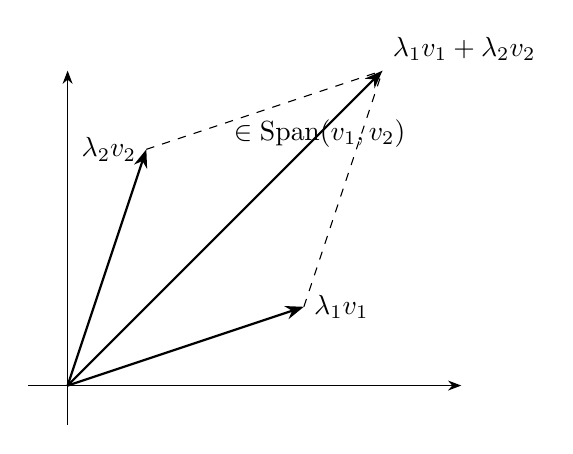
\begin{tikzpicture}[scale=1, >=Stealth]
\draw[->] (-0.5,0) -- (5,0);
\draw[->] (0,-0.5) -- (0,4);

\coordinate (v1) at (3,1);
\coordinate (v2) at (1,3);

\draw[->, thick] (0,0) -- (v1) node[right] {$\lambda_1 v_1$};
\draw[->, thick] (0,0) -- (v2) node[left] {$\lambda_2 v_2$};

\draw[dashed] (v1) -- ($(v1)+(v2)$);
\draw[dashed] (v2) -- ($(v1)+(v2)$);

\draw[->, thick] (0,0) -- ($(v1)+(v2)$) node[above right] {$\lambda_1 v_1+\lambda_2 v_2$};

\node at (3.2,3.2) {$\in \operatorname{Span}(v_1,v_2)$};
\end{tikzpicture}
\end{center}
\end{example}

\begin{example}
Let 
\[
v_1=\begin{pmatrix}2\\1\end{pmatrix}, 
\quad 
v_2=\begin{pmatrix}4\\2\end{pmatrix}.
\]
Then \(v_2 = 2v_1\), so
\[
\operatorname{Span}(v_1)=\operatorname{Span}(v_2).
\]
\begin{center}
\begin{tikzpicture}[scale=1.1, >=Stealth]
\draw[->] (-3,0) -- (3,0);
\draw[->] (0,-3) -- (0,3);

\draw[thick] (-2.5,-1.25) -- (2.5,1.25);

\draw[->, thick] (0,0) -- (1,0.5) node[right] {$v_1$};
\draw[->, thick] (0,0) -- (2,1) node[right] {$v_2$};

\node at (1.8,-1.6) {$\operatorname{Span}(v_1)=\operatorname{Span}(v_2)$};
\end{tikzpicture}
\end{center}
\end{example}

\paragraph{Span in $\mathbb{C}^n$}
\begin{definition}
The span over \(\mathbb{C}\) of vectors \(v_1,\ldots,v_n\) is
\[Span_{\mathbb{C}}(v_1,\ldots,v_n)=\{\lambda_1 v_1 + \ldots + \lambda_n v_n : \lambda_i \in \mathbb{C}\}.\]
\end{definition}
\begin{example}
For example,
\[\begin{pmatrix}2i\\2\end{pmatrix} + i\begin{pmatrix}3\\1+i\end{pmatrix} \in \mathbb{C}^2.\]
\end{example}

\medskip
\noindent
So we distinguish between real and complex vector spaces:
\[
\mathbb{R}^n = \left\{\begin{pmatrix}x_1\\\vdots\\x_n\end{pmatrix} : x_i \in \mathbb{R}\right\},
\qquad
\mathbb{C}^n = \left\{\begin{pmatrix}x_1\\\vdots\\x_n\end{pmatrix} : x_i \in \mathbb{C}\right\}.
\]

\subsubsection{Standard Basis}

\begin{definition}
The standard basis for \(\mathbb{R}^n\) is the set \(\{e_1,\ldots,e_n\}\), where \(e_i\) is the \(i\)th standard basis vector.

\[\mathbb{R}^n = \left\{\begin{pmatrix}x_1\\\vdots\\x_n\end{pmatrix} : x_i \in \mathbb{R}\right\}\]

\[e_1 = \begin{pmatrix}1\\0\\\vdots\\0\end{pmatrix}, \quad \ldots \quad e_n = \begin{pmatrix}0\\\vdots\\0\\1\end{pmatrix}\]
\end{definition}

\medskip
\noindent
(Basis = span + linear independence)

\paragraph{Claim}
These vectors span \(\mathbb{R}^n\).

\begin{proof}
We show that any vector in \(\mathbb{R}^n\) can be written as a linear combination of \(e_1,\ldots,e_n\):
\[\begin{pmatrix}x_1\\\vdots\\x_n\end{pmatrix} = \begin{pmatrix}x_1\\0\\\vdots\\0\end{pmatrix} + \begin{pmatrix}0\\x_2\\\vdots\\0\end{pmatrix} + \cdots + \begin{pmatrix}0\\\vdots\\0\\x_n\end{pmatrix} = x_1 e_1 + x_2 e_2 + \cdots + x_n e_n.\]
\end{proof}

\begin{example}[Complex vs Real Span]
    \[\mathbb{C}^2 = \operatorname{Span}_{\mathbb{C}}(e_1,e_2)
    = \{z_1 e_1 + z_2 e_2 : z_1,z_2 \in \mathbb{C}\},\]
    where 
    \[e_1=\begin{pmatrix}1\\0\end{pmatrix}, \quad e_2=\begin{pmatrix}0\\1\end{pmatrix}.\]
    Here \(\dim_{\mathbb{C}}\mathbb{C}^2=2\) but \(\dim_{\mathbb{R}}\mathbb{C}^2=4\).
    Every complex scalar can be written as \(z_k=x_k+iy_k\) with \(x_k,y_k \in \mathbb{R}\). So
    \[\operatorname{Span}_{\mathbb{C}}(e_1,e_2) = \{(x_1+iy_1)e_1 + (x_2+iy_2)e_2 : x_1,x_2,y_1,y_2 \in \mathbb{R}\}.\]
    Separating real and imaginary parts,
    \[\operatorname{Span}_{\mathbb{C}}(e_1,e_2) = x_1 e_1 + x_2 e_2 + y_1 (i e_1) + y_2 (i e_2).\]
    Therefore,
    \[\operatorname{Span}_{\mathbb{C}}(e_1,e_2) = \operatorname{Span}_{\mathbb{R}}\left(
    \begin{pmatrix}1\\0\end{pmatrix},
    \begin{pmatrix}0\\1\end{pmatrix},
    \begin{pmatrix}i\\0\end{pmatrix},
    \begin{pmatrix}0\\i\end{pmatrix}
    \right).
    \]

    \begin{center}
    \begin{tikzpicture}[scale=1.2, >=Stealth]
    \draw[->] (-3,0) -- (3,0) node[right] {$\Re$};
    \draw[->] (0,-3) -- (0,3) node[above] {$\Im$};

    \draw[->, thick] (0,0) -- (2,0) node[below] {$1$};
    \draw[->, thick] (0,0) -- (0,2) node[left] {$i$};

    \node at (1.5,1.5) {$\mathbb{C}=\text{span}_{\mathbb{R}}(1,i)$};
    \end{tikzpicture}
    \end{center}
\end{example}


\subsubsection{Abstract Vector Spaces}
An abstract vector space is just a set with two operations:
vector addition \((v_1+v_2)\) and scalar multiplication \((\lambda v)\), where \(\lambda\) comes from a field \(k\), satisfying certain axioms.

\begin{definition}
    Let \(k\) be a field. A \textbf{vector space over \(k\)} is a set \(V\) together with two operations
    \[
    \begin{cases}
    v_1+v_2 \in V, \quad v_1,v_2 \in V,\\
    \lambda v \in V, \quad v \in V, \ \lambda \in k,
    \end{cases}
    \]
    satisfying 8 axioms.
\end{definition}

\paragraph{Axioms}
(1) Rules for addition
\[(v_1+v_2)+v_3 = v_1+(v_2+v_3)\]
There exists a zero vector \(0 \in V\) such that \(0+v=v\).
For every \(v \in V\), there exists \(-v \in V\).
\[u+v = v+u\]
(2) Rules for scalar multiplication
\[1\cdot v = v\]
\[\lambda_1(\lambda_2 v) = (\lambda_1\lambda_2)v\]
(3) Compatibility (distributive laws)
\[(\lambda_1+\lambda_2)v = \lambda_1 v + \lambda_2 v\]
\[\lambda(v_1+v_2) = \lambda v_1 + \lambda v_2\]

\begin{example}
Let \(K\) be a field. Then
\[K^n = \left\{\begin{pmatrix}x_1\\\vdots\\x_n\end{pmatrix} : x_i \in K\right\}\]
is a vector space over \(K\).
\end{example}

\begin{remark}
\[\operatorname{Span}_{\mathbb{Z}}(e_1,e_2) = \{\lambda_1 e_1 + \lambda_2 e_2 : \lambda_i \in \mathbb{Z}\}.\]
\end{remark}

\begin{center}
\begin{tikzpicture}[scale=1.2, >=Stealth]
\draw[->] (-0.5,0) -- (3,0);
\draw[->] (0,-0.5) -- (0,3);

\draw[->, thick] (0,0) -- (2,0) node[below] {$e_1$};
\draw[->, thick] (0,0) -- (0,2) node[left] {$e_2$};

\node at (1.4,1.4) {$\mathbb{R}^2$};
\end{tikzpicture}
\end{center}

\subsubsection{Examples of Vector Spaces}
\marginpar{14 January, 2026}

We now list important examples of vector spaces.

\paragraph{1. Coordinate spaces}
Let \(k\) be a field (\(k=\mathbb{R}\) or \(k=\mathbb{C}\)).
\[
k^n = \left\{\begin{pmatrix}x_1\\\vdots\\x_n\end{pmatrix} : x_i \in k\right\}
\]
is a vector space over \(k\).

The standard basis is
\[
e_1=\begin{pmatrix}1\\0\\\vdots\\0\end{pmatrix}, \ \ldots \ ,
e_n=\begin{pmatrix}0\\\vdots\\0\\1\end{pmatrix}.
\]

\paragraph{2. Polynomial spaces}
A polynomial is an expression
\[
f(x)=a_n x^n + a_{n-1}x^{n-1} + \cdots + a_1 x + a_0,
\quad a_i \in k.
\]

\[
P_n(k)=\{a_n x^n + \cdots + a_1 x + a_0 : a_i \in k\}
\]
is a vector space over \(k\).

Examples:
\[
1+x^2 \in P_2(\mathbb{R}), \qquad 1+i x^3 \in P_3(\mathbb{C}).
\]

The subscript must satisfy \(\deg(f)\le n\).

All polynomials:
\[
P_\infty = \{a_n x^n + \cdots + a_1 x + a_0 : a_i \in k, \ n\ge0\}.
\]

\[
P_0 \subseteq P_1 \subseteq P_2 \subseteq \cdots \subseteq P_\infty.
\]

A standard basis is \(\{1,x,x^2,\ldots,x^n\}\).  
Every \(f \in P_n\) can be written
\[
f=\lambda_0 + \lambda_1 x + \lambda_2 x^2 + \cdots + \lambda_n x^n.
\]

\paragraph{3. Matrix spaces}
\[
M_n(k)=\left\{\begin{pmatrix}
a_{11}&\cdots&a_{1n}\\
\vdots&\ddots&\vdots\\
a_{n1}&\cdots&a_{nn}
\end{pmatrix}: a_{ij}\in k\right\}
\]
is a vector space over \(k\).

Standard basis matrices:
\[
e_{11}=\begin{pmatrix}1&0&\cdots&0\\0&0&\cdots&0\\\vdots&\vdots&\ddots&\vdots\\0&0&\cdots&0\end{pmatrix},\quad
e_{12}=\begin{pmatrix}0&1&\cdots&0\\0&0&\cdots&0\\\vdots&\vdots&\ddots&\vdots\\0&0&\cdots&0\end{pmatrix}, \ \ldots
\]

\[
\dim M_n(k)=n^2.
\]

Example in \(M_2(\mathbb{R})\):
\[
\begin{pmatrix}1&2\\3&4\end{pmatrix}
=1e_{11}+2e_{12}+3e_{21}+4e_{22}.
\]

\paragraph{4. Function spaces}
Let \(D\) be a set and \(k\) a field.
\[
F(D,k)=\{f:D\to k\}
\]
is a vector space over \(k\).

When \(D=\mathbb{R}\) and \(k=\mathbb{R}\), functions are drawn with horizontal axis \(D\) and vertical axis \(k\).


\marginpar{16 January, 2026}
$F(D)$ is a function from $D$ to $K$, where $K = \mathbb{R}\:or\:\mathbb{C}$. No "standard basis" in general.

Standard basis if $D$ is a finite set $eg\:D=\{1,\ldots,n\}$.
\[(f \in F(D). f(1)=2,f(2)=4,\ldots,f(n)=2^n\]

Kronecker function: Let $x \in D$, $\delta_x \in F(D)$, defined by $\delta_x(y)=\left\{\begin{array}{ll}1&x=y\\0&x\ne y\end{array}\right.$
Then $\{\delta_x : x \in D\}$ is a standard basis of $F(D)$.

Standard basis :\((\delta_1,\ldots,\delta_n)\), for $F(\{1,\ldots,n\})$.

Remark: $\{\delta_x : x \in \mathbb{R}\} $ do not span $F(\mathbb{R})$.

Proof that $(\delta_1,\ldots,\delta_n)$ spans $F\{1,\ldots,n\}$. Take any
\[f \in F(D)\]
Find $a_1,\ldots,a_n \in K$ such that
\[f = a_1 \delta_1 + \ldots + a_n \delta_n\]
\[f(x), \quad x \in D = \{1,\ldots,n\}\]
\[g(1) = a_1\delta_1(1) + a_2 \delta_2(1) + \ldots + a_n \delta_n(1) = a_1\]

Claim: $a_k = f(K) \in K$
Claim: $f = \sum f(k) \delta_k$, where $f(k) \in K$ and $\delta_k$ is the basis vector.

Proof:
\[g(l) = f(1)\delta_1(l)+\ldots+f(l)\delta_l(l)+\ldots+f(n)\delta_n(l) = f(l)\]

Subspace criterion. Let $V$ be a vector space.
To check a subset $u \subseteq V$ is a vector space.
In principle need to checck:
1. $U$ is stable under addition $u,v \in U$ Hence $u+v \in U$.
2. $U$ is stable under scalar multiplication. $\lambda \in K, u \in U$ Hence $\lambda u \in U$.
3. 8 axioms hold in $U$.

Proposition. A subset $U \subseteq V$ is a vector space (8 axioms are true) if f:
(0) $U$ is not empty ($0 \in U$)
(1) $U$ is stable under addition: $u,v \in U \to u + v \in U$.
(2) $U$ is stable under scalar multiplication: $u \in U, \lambda \in K \to \lambda u \in U$.

\marginpar{January 19, 2026}
Subspaces
\begin{problem}[Subspace criterion]
    Let $A \in M_n(K)$ be a fixed matrix. Prove thet
    \[U = \{x \in K^n : Ax = \vec{0}\}\]
    is a subspace, null space or kernel.
\end{problem}
\begin{problem}[Subspace criterion 2]
    The set $U = \{Ax : x \in K^n\}$ is a subspace, image of A.
\end{problem}
\begin{problem}[Subspace criterion 3]
    Let $V = K$ (vector space of dim 1) show that the only 2 subspaces of $V$ are $\{0\}$ and $V$ itself.
\end{problem}
\begin{problem}[Subspace criterion 4]
    $Span(v_1,\ldots,v_n) = \{\lambda_1v_1 + \ldots + \lambda_nv_n : \lambda_1,\ldots,\lambda_n \in K\}$ is a subspace.
\end{problem}
\begin{problem}
    $Span(v_1, \ldots, v_n)$ is the smallest subspace c
\end{problem}

\marginpar{January 21, 2026}
\begin{problem}[$K = \mathbb{R}$]
    Is $v_i \begin{pmatrix}
        3\\5\\-5\end{pmatrix}$ in the space of $v_1 = \begin{pmatrix}
            1\\2\\1
    \end{pmatrix}, v_2 = \begin{pmatrix}
        2\\5\\4
    \end{pmatrix}, v_3 = \begin{pmatrix}
        1\\3\\6
    \end{pmatrix}$
    In otherwords: are there $x,y,z \in \mathbb{R}$ such that $v = xv_1 + yv_2 + zv_3$?
\end{problem}
\begin{problem}
    Is $f: 3x^2 + 5x - 5$ in the span of $f_1 = x^2 + 2x + 1, f_2 = 2x^2 + 5x + 4, f_3 = x^2 + 3x + 6$?
    \[f = xf_1 + yf_2 + zf_3\]
\end{problem}

Intersection, sums, direct sums.
$W$ vector space.
$U, V \subseteq W$ two subspaces.
Definition: $U \cap V = \{v \in W : v \in U \text{ and } v \in V\}$ smallest intersection $\{0\}$.

The union of 2 subspaces in NOT a subspace (in general).

$W = \mathbb{R}^2$ :
draw a cartesian plane with vertical being $V$ and horizontal being $U$ and draw the cross ($u+v$).
$U \cup V =$ cross, no quadrant, not a subspace

Sum of 2 subspaces:
$U + V = \{u + v : u \in U, v \in V\}$
line $U$ + line $V$ = plane

Propoisition: $U, V$ are subspaces of $W$. $U + V$ is a subspace.
U cannot rescale a vector space, therefore $U + U = U$.
Proof:
$\subseteq$: Let $u + u' \in U + U$ prove $u + u' \in U$. Yes subce $U$ is a subspace stable under addition.
$\supseteq$: Take $u \in U$, prove $u \in U + U$. $u = u + 0 \in U + U$.
Proof: subspace criterion.
(0) $0 \in U + V$ since $0 \in U, 0 \in V$.
(1) Stable under addition: let $w_1, w_2 \in U + V$. Prove $w_1 + w_2 \in U + V$.
\[w_1 = u_1 + v_1, u_1 \in U, v_1 \in V\]
\[w_2 = u_2 + v_2, u_2 \in U, v_2 \in V\]
\[w_1 + w_2 = (u_1 + u_2) + (v_1 + v_2)\]
\[u_1 + u_2 \in U, v_1 + v_2 \in V\]
\[w_1 + w_2 \in U + V\]
(2) Stable under scalar multiplication: let $w \in U + V, \lambda \in K$. Prove $\lambda w = \lambda u + \lambda v \in U + V$.

Prop: $U + V = span(U \cup V)$.
$U + V = $ smalles subspace containing $U \cup V$.
Proof:
$\subseteq$: Take $w \in U + V$ prove $w \in span(U \cup V)$.
\[w = u + v, u \in U, v \in V\]
Prove $w \in span(U \cup V)$. (You could also write it like $span(U,V)$ since line can be of both in $U$ or $V$). 
$\supseteq$: Take $w \in span(U \cup V)$ prove $w \in U + V$.
\[w = a_1 u_1 + \ldots + a_n u_n + b_1 v_1 + \ldots + b_m v_m\]
where $u_i \in U, v_j \in V, a_i,b_j \in K$.
\[w = (a_1 u_1 + \ldots + a_n u_n) + (b_1 v_1 + \ldots + b_m v_m)\]
\[w = u + v, u \in U + V\]

\marginpar{January 23, 2026}
\subsection{Direct sums}
$U, V$ subspaces in $W$ (ambiant space).
\begin{definition}
    $U$ and $V$ are in direct sum if $U \cap V = \{0\}$.
    Its a sum where the intersection is zero.
    Sum: \[U + V = \{u + v : u \in U, v \in V\}\]
    Now if $U \cap V = \{0\}$ we write $U \oplus V$, and $U,V \subseteq W$.
    Sol: $W = U \oplus V$ means $\begin{cases}
        W = U + V\\
        U \cap V = \{0\}
    \end{cases}$
    To prove $W = U \oplus V$,
    \begin{itemize}
        \item $W = U + V$, $\subseteq$ Let $w \in W$. Prove: there exist $u \in U$, $v \in V$ such that $w = u + v$.
        \item $U \cap V = \{0\}$. $\supseteq$ automatic. Pick $w \in \{0\}$. Prove $w \in U \cap V$. By assumption $w = 0$. Prove $w \in U$ and $w \in V$ hold by definition of subspace. Only need to show $U \cap V \subseteq \{0\}$. Let $w \in U$ and $w \in V$. Prove $w = 0$.
    \end{itemize}
\end{definition}
\begin{tabular}{c|c}
    Sets & Vector Spaces\\
    \hline
    intersection $A \cap B$ & intersection $U \cap V$\\
    union $A \cup B$ & union $U + V$\\
    Disjoint union $A \sqcup B$ and $A \cap B = \emptyset$ & Direct sum $U \cap V = \{0\}$
\end{tabular}
\begin{example}
    \[D = \{1,2,3,4,5\}\]
    \[A = \{1,2,3\}, B = \{4,5,6\}\]
    Then
    \[D = A \sqcup B\]
\end{example}

$\to$ function spaces
$F(d) = $ functions on D.
\[f \in F(D)\]
Example of a function: $f(1) = 2, f(2) = \sqrt{2}, f(3) = \pi...$
View $F(A)$ as a subspace of $F(D)$.
Claim: $F(A)$ can be "identified" with a subspace $U\:of\: F(D)$.
\[U = \{f : D \to \mathbb{R} : f(x) = 0, x \notin A\}\]


\section{Appendix}

\section{Solutions}
\begin{solution}
    A field with 2 elements can be constructed as follows:
    Let \(F = \{0, 1\}\) be a set with two elements. We define addition and multiplication operations on \(F\) as follows:
    \begin{itemize}
        \item \(0 + 0 = 0\)
        \item \(0 + 1 = 1\)
        \item \(1 + 0 = 1\)
        \item \(1 + 1 = 0\)
        \item \(0 \times 0 = 0\)
        \item \(0 \times 1 = 0\)
        \item \(1 \times 0 = 0\)
        \item \(1 \times 1 = 1\)
    \end{itemize}
\end{solution}
\begin{solution}
    Suppose \(B\) and \(B'\) are both inverses of \(A\). Then
    \[B = B I = B(AB') = (BA)B' = I B' = B'.\]
    Therefore, \(B = B'\), so the inverse is unique.
\end{solution}
\begin{solution}
    We can answer this problem with proof by contradiction. Let's
    suppose this matrix is invertible. By definition there exists B = $\begin{pmatrix}a&b\\c&d\end{pmatrix}$ such that $\begin{bmatrix}0&1\\0&0\end{bmatrix}$ $\begin{bmatrix}a&b\\c&d\end{bmatrix}$ = $\begin{bmatrix}1&0\\0&1\end{bmatrix}$.  We can rewrite this equation into: $\begin{bmatrix}a&b\\c&d\end{bmatrix}$ = $\begin{bmatrix}0&1\\0&0\end{bmatrix}^{-1}$. The inverse of our matrix can be rewritten as $\frac{1}{0*0 - 1*0}\begin{bmatrix}0&-1\\0&0\end{bmatrix}$\footnote{Recall that an inverse of a $2 \times 2$ matrix is equal to its determinant multiplied with its conjugate}. But this is undefined since division by 0 is undefined. Therefore, our initial assumption that the matrix is invertible is false, and thus the matrix is not invertible.
\end{solution}
\begin{solution}[Subspace criterion]
    (0) is $0 \in U$?
    Yes, because $A0 = 0$.
    \[\begin{pmatrix}
        a&b\\
        c&d
    \end{pmatrix}\begin{pmatrix}
        0\\0
    \end{pmatrix} = \begin{pmatrix}
        0\\0
    \end{pmatrix}\]
    
    (1) Addition: Let $x,y \in U$. Prove $x+y \in U$.
    \[A(x+y) = Ax + Ay = 0 + 0 = 0\]
    (2) Scalar multiplication: Let $x \in U, \lambda \in K$. Prove $\lambda x \in U$.
    \[A(\lambda x) = \lambda Ax = \lambda 0 = 0\]
\end{solution}
\begin{solution}[Subspace criterion 2]
    (0) is $0 \in U$?
    Find $x \in K^n$ such that $Ax = 0$.
    $x = 0$.

    (1) Stability under addition: $y_1,y_2 \in U \to y_1 + y_2 \in U$.
    There exist $x$, such that $y_1 = Ax_1, y_2 = Ax_2$.
    \[y_1 + y_2 = Ax_1 + Ax_2 = A(x_1 + x_2) \in U\]
    
    (2) Stability under scalar multiplication: If $f = Ax$, for some $x$, $\lambda y = A(\lambda x)$
\end{solution}
\begin{solution}[Subspace criterion 3]
    Let $U \subseteq \mathbb{R}$ be a subspace. Prove: $U = \{0\}$ or $U = \mathbb{R}$.
    
    Case 1: $U = \{0\}$.

    Case 2: $U \ne \{0\} \to$ there exists $v \in \mathbb{R}$, $v \ne 0$.
    Prove: $U = \mathbb{R}$.
    Let $x \in \mathbb{R}$ be any real number. Prove: $x \in U$.
    Since $U$ is a subspace, it is stable under scalar multiplication.
    \[x \in U \to Ax \in U\]
    Therefore, $x \in U$.
\end{solution}
\begin{solution}[Subspace criterion 4]
    (0) $0 \in span(v_1,\ldots,v_n)$, because
    \[\lambda_1 = \ldots \lambda_n = 0 \qquad \lambda_1 v_1 + \ldots + \lambda_n v_n = 0.\]
    
    (1) addition: $u,v \in span$ Prove $u + v \in span$.
    \[u = a_1 v_1 + \ldots + a_n v_n\]
    \[v = b_1 v_1 + \ldots + b_n v_n\]
    \[u + v = (a_1 + b_1)v_1 + \ldots + (a_n + b_n)v_n \in span(v_1,\ldots,v_n)\]
    
    (2) scalar multiplication:
\end{solution}
\begin{solution}
    \[\begin{pmatrix}
        3\\5\\-5
    \end{pmatrix} = x\begin{pmatrix}
        1\\2\\1
    \end{pmatrix} + y\begin{pmatrix}
        2\\5\\4
    \end{pmatrix} + z\begin{pmatrix}
        1\\3\\6
    \end{pmatrix}\]
    \[\begin{cases}
        x+2y+z = 3\\
        2x+5y+3z = 5\\
        x+4y+6z = -5
    \end{cases} \to x = 3, y = 1, z = -2\]
    A: yes since 
    \[v = 3v_1 + v_2 + 2v_3\]
\end{solution}

\section{Useful Links}

\end{document}